\documentclass{article}
\usepackage{tikz}
\usepackage{pgfplots}
\usepackage{amsmath, amsfonts}
\usepackage{enumerate}
\usepackage{pdfpages}
\input{title.tex}

\newcommand{\N}{\mathbb{N}}
\newcommand{\R}{\mathbb{R}}
\newcommand{\E}{\mathbb{E}}
\newcommand{\V}{\mathbb{V}}
\renewcommand{\P}{\mathbb{P}}
\begin{document}
    \maketitle
    \section{}
    \begin{enumerate}[a)]
        \item Es wurden 100 Sitze reserviert.
        \item Es wurden insgesamt $65 + 62 = 127$ Sitze reserviert.
        \item Problem: Es wurden einige Sitze doppelt reserviert. Es findet eine Art Race Condition statt:
            Beide Threads rufen unabhängig voneinander die Funktionen \verb|reserve()|, \verb|reserveSeat()| und
            \verb|payment()| auf. Es kann bspw. vorkommen, dass Thread 1 im gemeinsamen Array \verb|seats|
            (in der Funktion \verb|reserveSeat()|) gerade den Sitz 44 als frei erkannt hat (\verb|freeSeat = false|) (was durch die
            for-Schleife außerdem bedeutet, dass die Sitze 0 bis 43 bereits reserviert sind).
            Und während der dabei ist, den Sitz zu reservieren und \verb|payment()| aufzurufen, greift Thread 2 ebenfalls
            auf den Sitz 44 zu, da der immernoch als false (also nicht reserviert) im Array steht. Thread 2
            arbeitet dann quasi auf einem veralteten Wert und reserviert den Sitz 44 ebenfalls.
            \\ Im Wesentlichen sind die Codezeilen das Problem, in denen auf \verb|seats| zugegriffen wird; also:
            Zeilen 33 bis 38.
        \item \begin{enumerate}[i.]
            \item Da man beliebig viele Threads erstellen kann, ist diese Eigenschaft nicht erfüllt.
                Im worst case wird jeder Sitz durch jeden Thread einmal reserviert, d.h. bei 3 Threads wären
                das z.B. 300 Sitze. (Falls allerdings nur gemeint ist, ob die Eigenschaft mit 2 Threads erfüllt ist,
                dann wäre die Antwort Ja.)
            \item Das ist nicht erfüllt; siehe c) für ein Gegenbeispiel.
            \item Das ist erfüllt, denn die while-Schleife in der run() Methode läuft für jeden Thread solange
                \verb|reserve()| erfolgreich war; was aber immer passiert, wenn mindestens ein Sitz noch als frei (false)
                in \verb|seats| steht. (Genauer: Der Rückgabewert von \verb|reserve()| entspricht der Variablen
                \verb|seatReserved|, die wiederum der Rückgabe von \verb|reserveSeat(i)| entspricht. \verb|reserveSeat(i)| gibt
                genau dann true zurück, wenn \verb|seats[i] = false| ist (also Sitz i frei ist). Die for-Schleife in Zeile 17
                läuft solange, bis ein Sitz reserviert wurde und gibt dann true aus; oder gibt false aus, wenn kein Sitz mehr frei ist.)
            \item Das ist ebenfalls erfüllt. Wie oben erläutert, gibt \verb|reserve()| immer true zurück, wenn ein Sitz
                in \verb|seats| frei war und reserviert werden konnte. In der for-Schleife wird das ja für jeden Sitz geprüft;
                nur wenn \verb|seats[i] = true| $\forall$\verb|i|$\in [0, 99]$ gilt, dann wird auch kein Sitz reserviert.
        \end{enumerate}
        \item Das ist erfüllt. Für jeden Zustand des Programms gilt, dass entweder noch mind. ein Eintrag in \verb|seats| existiert,
            der false ist (1), oder alle Einträge in \verb|seats| true sind (2). In Fall (1) wird dieser Eintrag innerhalb der
            for-Schleife in Zeile 17 gefunden werden und dann gibt \verb|reserveSeat()| aus, dass ein Sitz reserviert wurde.
            Tritt Fall (2) ein, dann wird nach der for-Schleife ausgegeben, dass kein Sitz reserviert werden konnte.
    \end{enumerate}
    \section{}
    \begin{enumerate}[a)]
        \item
            \begin{enumerate}[i.]
                \item
                    Registermaschine:\\
                    \begin{tabular}{l|l}
                        \multicolumn{2}{l}{
                            $\pi$
                        }\\
                        \hline
                        \multicolumn{2}{l}{
                            load R1, 0x00
                        }\\
                        \multicolumn{2}{l}{
                            store R1, n
                        }\\
                        \hline
                        p:&q:\\
                        load R1, n&load R1, n\\
                        add R1, 0x01&sub R1, 0x01\\
                        store R1, n&store R1, n
                    \end{tabular}\\
                    Stapelmaschine:\\
                    \begin{tabular}{l|l}
                        \multicolumn{2}{l}{
                            $\pi$
                        }\\
                        \hline
                        \multicolumn{2}{l}{
                            push 0
                        }\\
                        \multicolumn{2}{l}{
                            pop n
                        }\\
                        \hline
                        p:&q:\\
                        push n&push n\\
                        push 1&push1\\
                        add&sub\\
                        pop n&pop n
                    \end{tabular}
                \item
                    Korrekter Ablauf $n=0$ zum Ende.
                    Registermaschine:\\
                    \begin{tabular}{cl|l}
                        thread&Programm & n\\
                        \hline
                        &load R1, 0x00&UNDEF\\
                        &store R1, n&0\\
                        p&load R1, n&0\\
                        p&add R1, 0x01&0\\
                        p&store R1, n&1\\
                        q&load R1, n&1\\
                        q&sub R1, 0x01&1\\
                        q&store R1, n&0\\
                    \end{tabular}
                    Stapelmaschine:
                    \begin{tabular}{cl|l}
                        thread&Programm & n\\
                        \hline
                        &push 0&UNDEF\\
                        &pop n&0\\
                        p&push n&0\\
                        p&push 1&0\\
                        p&add&0\\
                        p&pop n&1\\
                        q&push n&1\\
                        q&push 1&1\\
                        q&sub&1\\
                        q&pop n&0\\
                    \end{tabular}\\
                    Inkorrekter Ablauf $(n\neq 0)$ zum Ende.
                    Registermaschine:\\
                    \begin{tabular}{cl|l}
                        thread&Programm & n\\
                        \hline
                        &load R1, 0x00&UNDEF\\
                        &store R1, n&0\\
                        p&load R1, n&0\\
                        q&load R1, n&0\\

                        q&sub R1, 0x01&0\\
                        p&add R1, 0x01&0\\
                        q&store R1, n&-1\\
                        p&store R1, n&1\\
                    \end{tabular}
                    Stapelmaschine:
                    \begin{tabular}{cl|l}
                        thread&Programm & n\\
                        \hline
                        &push 0&UNDEF\\
                        &pop n&0\\
                        p&push n&0\\
                        p&push 1&0\\
                        p&add&0\\
                        q&push n&0\\
                        q&push 1&0\\
                        q&sub&0\\
                        q&pop n&-1\\
                        p&pop n&1\\
                    \end{tabular}
            \end{enumerate}
        \item
            $\{4, 8, 12,\hdots,40\}$
        \item
            \begin{enumerate}[i.]
                \item $(8, 0)$
                \item $(8, 0)$
            \end{enumerate}
    \end{enumerate}
    \section{}
    \begin{enumerate}[a)]
        \item
            \begin{enumerate}[i.]
                \item
                    Wenn $p_2$, sowie $q_2$ gleichzeitig ausgeführt werden.
                \item
                    \begin{itemize}
                        \item
                            Beide Prozesse dürfen nicht gleichzeitig auf $R$ zugreifen.\\
                            Ist keine zwar eine Sicherheitseigenschaft, aber keine gute,
                            da sie ambiguos ist. Besser wäre ``Beide prozesse greifen
                            nicht gleichzeitig auf $R$ zu.''\\
                            Es handelt sich um eine Sicherheitseigenschaft, da eine Invariante
                            beschrieben wird.
                        \item
                            In jedem Zustand gibt es eine Fortsetzung, in der ein Prozess
                            schließlich auf $R$ zugreifen kann.\\
                            Es handelt sich um eine Lebendigkeitseigenschaft, da
                            gewährleistet wird, dass die Eigenschaft ``Zugriff auf $R$''
                            in endlich vielen Schritten (schließlich) gewähleistet wird.
                    \end{itemize}
            \end{enumerate}
        \item
            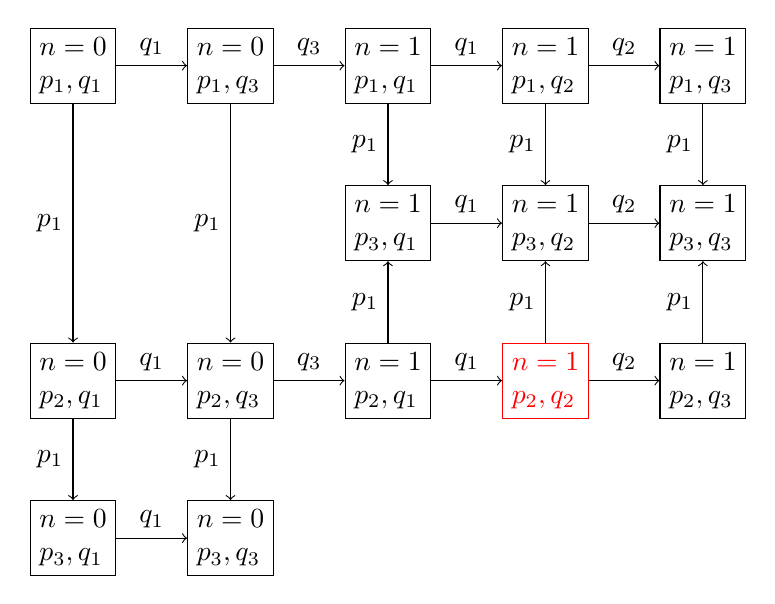
\begin{tikzpicture}
                \node[draw, align=left] (011) at (0,0) {$n=0$\\$p_1,q_1$};
                \node[draw, align=left] (013) at (2,0) {$n=0$\\$p_1,q_3$};
                \node[draw, align=left] (021) at (0,-4) {$n=0$\\$p_2,q_1$};
                \node[draw, align=left] (023) at (2,-4) {$n=0$\\$p_2,q_3$};
                \node[draw, align=left] (031) at (0,-6) {$n=0$\\$p_3,q_1$};
                \node[draw, align=left] (033) at (2,-6) {$n=0$\\$p_3,q_3$};


                \node[draw, align=left] (111) at (4,0) {$n=1$\\$p_1,q_1$};
                \node[draw, align=left] (112) at (6,0) {$n=1$\\$p_1,q_2$};
                \node[draw, align=left] (113) at (8,0) {$n=1$\\$p_1,q_3$};
                \node[draw, align=left] (121) at (4,-4) {$n=1$\\$p_2,q_1$};
                \node[draw, align=left, color=red] (122) at (6,-4) {$n=1$\\$p_2,q_2$};
                \node[draw, align=left] (123) at (8,-4) {$n=1$\\$p_2,q_3$};
                \node[draw, align=left] (131) at (4,-2) {$n=1$\\$p_3,q_1$};
                \node[draw, align=left] (132) at (6,-2) {$n=1$\\$p_3,q_2$};
                \node[draw, align=left] (133) at (8,-2) {$n=1$\\$p_3,q_3$};

                \draw[->]
                    (011) edge[above] node{$q_1$} (013)
                    (013) edge[above] node{$q_3$} (111)
                    (021) edge[above] node{$q_1$} (023)
                    (023) edge[above] node{$q_3$} (121)
                    (031) edge[above] node{$q_1$} (033)
                    (111) edge[above] node{$q_1$} (112)
                    (112) edge[above] node{$q_2$} (113)
                    (121) edge[above] node{$q_1$} (122)
                    (122) edge[above] node{$q_2$} (123)
                    (131) edge[above] node{$q_1$} (132)
                    (132) edge[above] node{$q_2$} (133)

                    (011) edge[left] node{$p_1$} (021)
                    (013) edge[left] node{$p_1$} (023)
                    (021) edge[left] node{$p_1$} (031)
                    (023) edge[left] node{$p_1$} (033)
                    (111) edge[left] node{$p_1$} (131)
                    (112) edge[left] node{$p_1$} (132)
                    (113) edge[left] node{$p_1$} (133)
                    (121) edge[left] node{$p_1$} (131)
                    (122) edge[left] node{$p_1$} (132)
                    (123) edge[left] node{$p_1$} (133)
                    ;
            \end{tikzpicture}\\
            Da es sich bei den Paaren $((n=0,p_i,q_j),(n=2,p_i,q_j))_{i,j\in\{1,2,3\}}$ jeweils
            um äquivalente Zustände handelt ($2\equiv 0\mod 2$) gibt es von jedem zustand
            einen Pfad zu einem Zustandspaar mit $q_2$ und $p_2$.
            Demnach ist Eigenschaft 2 gewährleistet.
            Eigenschaft 1 gilt nicht bei Zustand $(n=0,p_2,q_2)$
        \item
            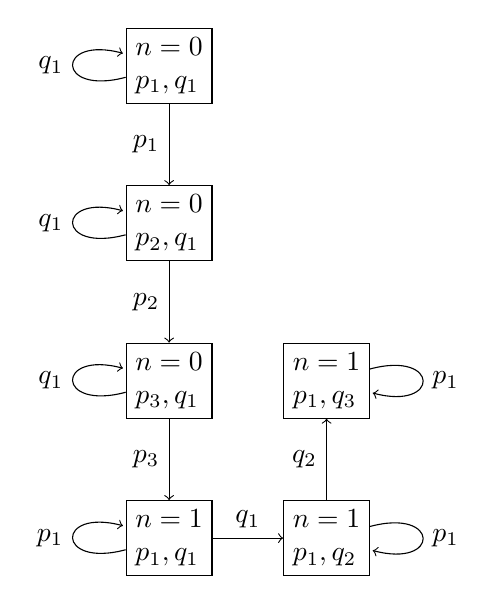
\begin{tikzpicture}
                \node[draw, align=left] (011) at (0,0) {$n=0$\\$p_1,q_1$};
                \node[draw, align=left] (021) at (0,-2) {$n=0$\\$p_2,q_1$};
                \node[draw, align=left] (031) at (0,-4) {$n=0$\\$p_3,q_1$};
                \node[draw, align=left] (111) at (0,-6) {$n=1$\\$p_1,q_1$};
                \node[draw, align=left] (112) at (2,-6) {$n=1$\\$p_1,q_2$};
                \node[draw, align=left] (113) at (2,-4) {$n=1$\\$p_1,q_3$};
                \draw[->]
                    (011) edge[loop left] node{$q_1$} (011)
                    (021) edge[loop left] node{$q_1$} (021)
                    (031) edge[loop left] node{$q_1$} (031)
                    (111) edge[loop left] node{$p_1$} (111)
                    (112) edge[loop right] node{$p_1$} (112)
                    (113) edge[loop right] node{$p_1$} (113)

                    (011) edge[left] node{$p_1$} (021)
                    (021) edge[left] node{$p_2$} (031)
                    (031) edge[left] node{$p_3$} (111)

                    (112) edge[left] node{$q_2$} (113)

                    (111) edge[above] node{$q_1$} (112)
                    ;
            \end{tikzpicture}\\
            Mit selber Begründung wie b) gilt auch hier wieder Eigenschaft 2.
            Anders als in b) gilt hier Eigenschaft 1, da es keinen Zustand mit
            $p_2$ und $q_2$ gibt.
    \end{enumerate}
    \section{}
    \begin{enumerate}[a)]
        \item
            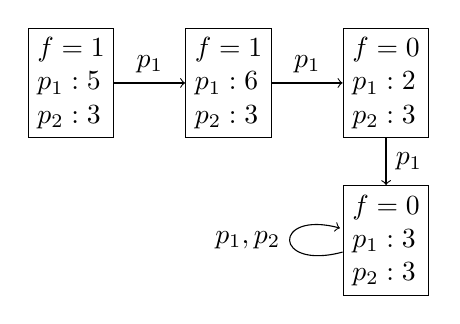
\begin{tikzpicture}
                \node[draw, align=left] (a) at (0,0) {$f=1$\\$p_1:5$\\$p_2:3$};
                \node[draw, align=left] (b) at (2,0) {$f=1$\\$p_1:6$\\$p_2:3$};
                \node[draw, align=left] (c) at (4,0) {$f=0$\\$p_1:2$\\$p_2:3$};
                \node[draw, align=left] (d) at (4,-2){$f=0$\\$p_1:3$\\$p_2:3$};
                \draw[->]
                    (a) edge[above] node{$p_1$} (b)
                    (b) edge[above] node{$p_1$} (c)
                    (c) edge[right] node{$p_1$} (d)
                    (d) edge[loop left] node{$p_1,p_2$} (d)
                    ;
            \end{tikzpicture}\\
            Nach diesem Ablauf der Zustände sind sowohl $p_1$, wie auch
            $p_3$ in der \verb|while testAndSet(flag)|-Schleife gefangen,
            da diese für \verb|flag| (=1) 1 zurückgibt.
        \item
            \begin{tabular}{l|l|l}
                \verb|flag|&$p_1$&$p_2$\\
                \hline
                0&\verb|doSomething|\\
                0&\verb|testAndSet(flag)|\\
                1&\verb|doSomethingElse|\\
                1&&\verb|doSomething|\\
                1&&enter \verb|testAndSet(flag)|\\
                1&&\verb|oldValue|$\leftarrow$\verb|1|\\
                0&\verb|flag|$\leftarrow$\verb|0|\\
                0&&\verb|if flag = 0| (true)\\
                1&&\verb|flag|$\leftarrow$\verb|1|\\
                1&&\verb|return 1|\\
                1&&\verb|while 1 = 1 do|\\
                1&\verb|doSomething|\\
                1&\verb|while testAndSet(flag) = 1|&\verb|while testAndSet(flag) = 1|
            \end{tabular}\\
            Da \verb|testAndSet(1)| = 1 sind beide Prozesse, in der inneren Schleife gefangen,
            $p_2$ führt \verb|doSomethingElse| nie aus.
    \end{enumerate}
\end{document}
